\documentclass[12pt]{article}
\setlength\parindent{0pt}
\usepackage{fullpage}
\usepackage[margin=0.5in]{geometry}
\usepackage{amsmath}
\usepackage{pdflscape}
\usepackage{graphicx}
\setlength{\parskip}{4mm}
\def\LL{\left\langle}   % left angle bracket
\def\RR{\right\rangle}  % right angle bracket
\def\LP{\left(}         % left parenthesis
\def\RP{\right)}        % right parenthesis
\def\LB{\left\{}        % left curly bracket
\def\RB{\right\}}       % right curly bracket
\def\PAR#1#2{ {{\partial #1}\over{\partial #2}} }
\def\PARTWO#1#2{ {{\partial^2 #1}\over{\partial #2}^2} }
\def\PARTWOMIX#1#2#3{ {{\partial^2 #1}\over{\partial #2 \partial #3}} }
\newcommand{\BE}{\begin{displaymath}}
\newcommand{\EE}{\end{displaymath}}
\newcommand{\BNE}{\begin{equation}}
\newcommand{\ENE}{\end{equation}}
\newcommand{\BEA}{\begin{eqnarray}}
\newcommand{\EEA}{\nonumber\end{eqnarray}}
\newcommand{\EL}{\nonumber\\}
\newcommand{\la}[1]{\label{#1}}
\newcommand{\ie}{{\em i.e.\ }}
\newcommand{\eg}{{\em e.\,g.\ }}
\newcommand{\cf}{cf.\ }
\newcommand{\etc}{etc.\ }
\newcommand{\Tr}{{\rm tr}}
\newcommand{\etal}{{\it et al.}}
\newcommand{\OL}[1]{\overline{#1}\ } % overline
\newcommand{\OLL}[1]{\overline{\overline{#1}}\ } % double overline
\newcommand{\OON}{\frac{1}{N}} % "one over N"
\newcommand{\OOX}[1]{\frac{1}{#1}} % "one over X"

\pagenumbering{gobble}

\begin{document}
\Large
\centerline{\sc{Recitation Exercises}}
\normalsize
\centerline{\sc{April 20}}
%
%\centerline{\large Question 1: rotational dynamics fundamentals}
%
%\vspace{1in}
%
%  A light cable is wound around a cylindrical spool fixed in place of radius 50 cm and mass 10 kg. One end of the cable is attached to a motor, which pulls with a constant force of 20 N on the cable. When the motor is switched on, the force exerted by the cable causes the spool to rotate faster and faster.
%\begin{enumerate}
%      \item{What is the moment of inertia of the spool?}
%\vspace{0.7in}
%      \item{What is the torque applied to the spool by the motor?}
%\vspace{0.7in}
%      \item{What is the angular acceleration of the spool?}
%\vspace{0.7in}
%      \item{How long will it take for the spool to make a full revolution?}
%\vspace{0.7in}
%      \item{After five seconds, how fast is the cable moving?}
%\vspace{0.7in}
%      \item{After five seconds, what is the kinetic energy of the spool?}
%\vspace{0.7in}
%      \item{What is the work done by the motor in five seconds?}
%     \end{enumerate}
%\newpage

\centerline{\large Question 1: torque and mechanical advantage}

\begin{minipage}{0.45\textwidth}
An engineering student constructs a crude balance scale out of a meter stick and a mass. They attach a supporting rod to the 50cm mark at the center of the meter stick (about which it is free to pivot), attach a movable one-kilogram mass to the left side, and
tie a string to the far end of the meter stick. (Suppose that the left side is the 0 cm mark, so the string is tied at the 100 cm mark.) 
\end{minipage}
\begin{minipage}{0.55\textwidth}
	\begin{center}
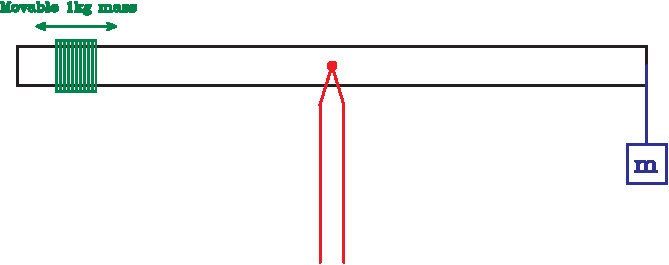
\includegraphics[width=3.5in]{balance-scale-crop.pdf}
\end{center}
\end{minipage}
\bigskip



To measure an unknown mass, you tie the unknown mass to the string at the right side, then slide the mass on the left back and forth until the meter stick is balanced and does not tip one way or the other. \textit{(This happens when the net torque on it is zero.)}



a) Draw an extended force diagram for the meter stick. \textit{(This means you should draw not just a dot, but the entire object. Then label each force at the position where it acts.)}

\vspace{3in}

b) In analyzing the torques on this system, you'll need to choose a pivot. It is a good idea to choose the pivot at the location of forces that you {\bf do not know} and {\bf do not care about}. What location should you choose? Label this position on your force diagram.

\vspace{1in}

\newpage

c) Suppose the system is balanced when you put the movable mass on the 20cm mark. What is the unknown mass?

\vspace{2in}

d) Another engineering student comes by and wants to modify the device, since they need to measure masses more than 1kg. They shift the support rod to the 80 cm mark. Draw an extended force diagram for the rod now.

\vspace{2in}

e) Referencing the idea of torque, explain in words why this will let you measure heavier masses than attaching the rod to the 50cm mark. Once your group has an explanation, call one of your instructors over and share your explanation with them.

\vspace{1.5in}

f) Another engineering student comes by and says ``Wait, you won't get very precise measurements out of this unless you measure the mass of the meter stick, too.'' Why does the mass of the meter stick not matter when the support rod is attached at the 50 cm mark, but does matter when it is attached at the 80 cm mark?


\newpage


\centerline{\large Question 2: on static equilibrium}



\begin{minipage}[b]{0.4\textwidth}
  \vspace{-0.8in}

A 4m-long pole of mass 80 kg extends from the side of a building, angled at 60 degrees above the horizontal. One meter from the end of the pole, a sign of mass 50 kg is attached. To support the pole,
a horizontal cable runs from the end of the pole to the building. (See the attached figure.)

\bigskip
\bigskip
\bigskip
\bigskip
\bigskip
\bigskip

\end{minipage}
\begin{minipage}[t]{0.6\textwidth}
  \begin{flushright}
  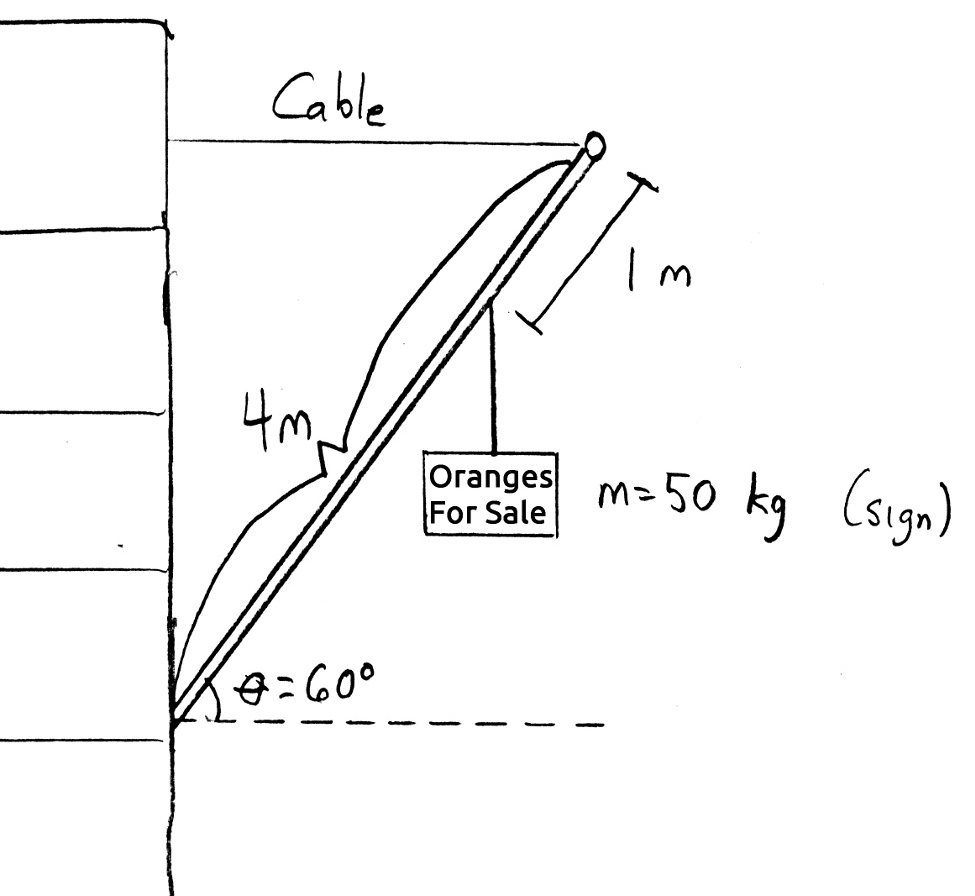
\includegraphics[width=0.9\textwidth]{sign2.jpg}
\end{flushright}
\end{minipage}

\bigskip
\bigskip

\newpage

a) Draw a force diagram, showing all of the elements needed to help you compute the tension in the support cable. Indicate
your choice of pivot point.

\vspace{5in}

\newpage

\begin{landscape}

b) Complete the following table, letting you calculate the torque from every force in the problem. 

\Large
\begin{center}
\begin{tabular}{|c|c|c|c|c|c|}
\hline
Name & Distance to pivot ($r$) & Size of force (F) & $\sin \theta$ & + or - & {\bf Torque} \\
     & & & (angle between $\vec F$ and $\vec r$) & & \\\hline
              &                         &                        &                                              &                    &                               \\ \hline
              &                         &                        &                                              &                    &                               \\ \hline
              &                         &                        &                                              &                    &                               \\ \hline
              &                         &                        &                                              &                    &                               \\ \hline
\end{tabular}
\end{center}
\normalsize
c) Compute the tension in the cable.

\vspace{3 in}

d) Suppose now that the store owner wanted to attach the cable to a different point on the building in order to minimize its tension. What angle between the
cable and the horizontal would support the pole with the minimum tension?
\end{landscape} \newpage


\newpage

\centerline{\large Question 3: torque in dynamic equilibrium}

A unicyclist rides at a constant speed of 5 m/s; she and her unicycle have a combined mass of 70 kg. The wheel of her unicycle has a radius of 50 cm. At this speed, air resistance exerts a force of 80 N on her.


1) What is the angular velocity of the wheel?
\vspace{1.2in}

2) As you know, the force that wheeled vehicles use to propel themselves forward is static friction. What is the size of this force?
\vspace {1.2in}

3) What torque must she apply to the wheel to maintain her speed? \textit{(Hint: What is the net torque on the wheel?)}
\vspace{2in}

\newpage

4) Suppose the pedals are attached to a crank with a radius of 25 cm. What force must she apply to the pedals to maintain her speed?
\vspace{3in}

5) What power does she apply to the pedals? What power does the air resistance apply?
\newpage

\Large
\centerline{\sc{Recitation Exercises}}
\normalsize
\centerline{\sc{April 22}}


\centerline{\large Question 1: on rotational dynamics}
A flywheel (a large, spinning disc) of mass $m$ and radius $r$ is rotating
at angular velocity $\omega$. The machine operator wishes to bring it to rest using a friction brake. When the brake
is engaged, two brake pads on either side of the disc are pressed against it from either side, two-thirds
of the way from the center to the outer edge; each brake pad
exerts a normal force $F_N$.

If the coefficient of friction between the brake pads and the disc is $\mu_k$, how long does it take the
brake to bring the flywheel to a stop?

\newpage
\centerline{\large Question 2: on linked objects}

A bucket of mass $m$ hangs from a string wound around a pulley
(a solid cylinder) with mass $M$ and radius $r$. When the bucket is
released, it falls, unwinding the string.

\begin{enumerate}

\item Draw force diagrams for the bucket and the pulley. Note that since the pulley rotates, you will need
to draw an extended force diagram for it, drawing the object and labeling where each force acts.

\vspace{3in}

\item In terms of the forces in your force diagrams, write an expression for the net torque on the pulley.

\vspace{1in}

\item Write down Newton's laws of motion -- $\sum \vec F = m \vec a$ for translation, and $\sum \tau = I \alpha$
-- for each object. (One object moves, and the other turns...)

\vspace{2in}


\newpage

\item What is the relationship between the angular acceleration $\alpha$ of the pulley and the linear acceleration
$a$ of the bucket? (The answer may be different depending on how you have drawn your pictures and your choice of
coordinate system.)

\vspace{1in}

\item Calculate the acceleration of the bucket in terms of $m$ and $M$.

\vspace{3in}

\item Suppose that the pulley were a hollow cylinder with the same mass. How would this acceleration change?

\end{enumerate}
\end{document}
